\section{El modelo Transformer}

A finales del año 2017 se presentó un nuevo modelo que vino a revolucionar el área de Procesamiento
de Lenguaje Natural, El Transformer \cite{Vaswani}. Una de sus principales características es la
capacidad de procesar la información de alguna secuencia de forma paralela, caso contrario a las
Redes Neuronales Recurrentes, donde la información se procesa recurrentemente. Gracias a ello,
la capacidad de \textit{recuerdo} no se ve afectado por el problema de \textit{El desvanecimiento
del Gradiente} específicamente cuando el problema es trabajar con secuencias  bastante largas.

\textit{El Transformer} puede ser visto como otro modelo \textit{seq2seq} (Secuencia a Secuencia)
\ref{fig:trans_seq2sqe}, formado en por dos etapas, la primera encargada de codificar la información de entrada
y la segunda de decodificarla, pero su principal característica es que aplica mecanismos de
\textit{Self-Attention} para capturar las dependencias globales entre la entrada y la salida. Dada
una secuencia de entrada $X = (x_1, x_2, \dots, x_n )$ con $n$ como el tamaño de la secuencia,
el codificador produce una representación intermedia
$Z = (z_1, z_2, \dots, z_n)$ al igual que los modelos \textit{seq2seq}. El decodificador usa la
secuencia $Z$ para generar la secuencia de salida
$Y = (y_1, y_2, \dots, y_m)$ uno a la vez (en modo inferencia), con $m$ como el tamaño de la
secuencia de salida. Nótese, que el generar una salida a la vez el decodificador tiene que ser auto-regresivo.
Usa la salida anterior $y_{i-1}$ como entrada adicional para generar la siguiente salida $y_i$. Por
ello, durante entrenamiento el modelo es alimentado con entradas y salidas desfasadas en un tiempo.

\begin{figure}[ht!]
    \centering
    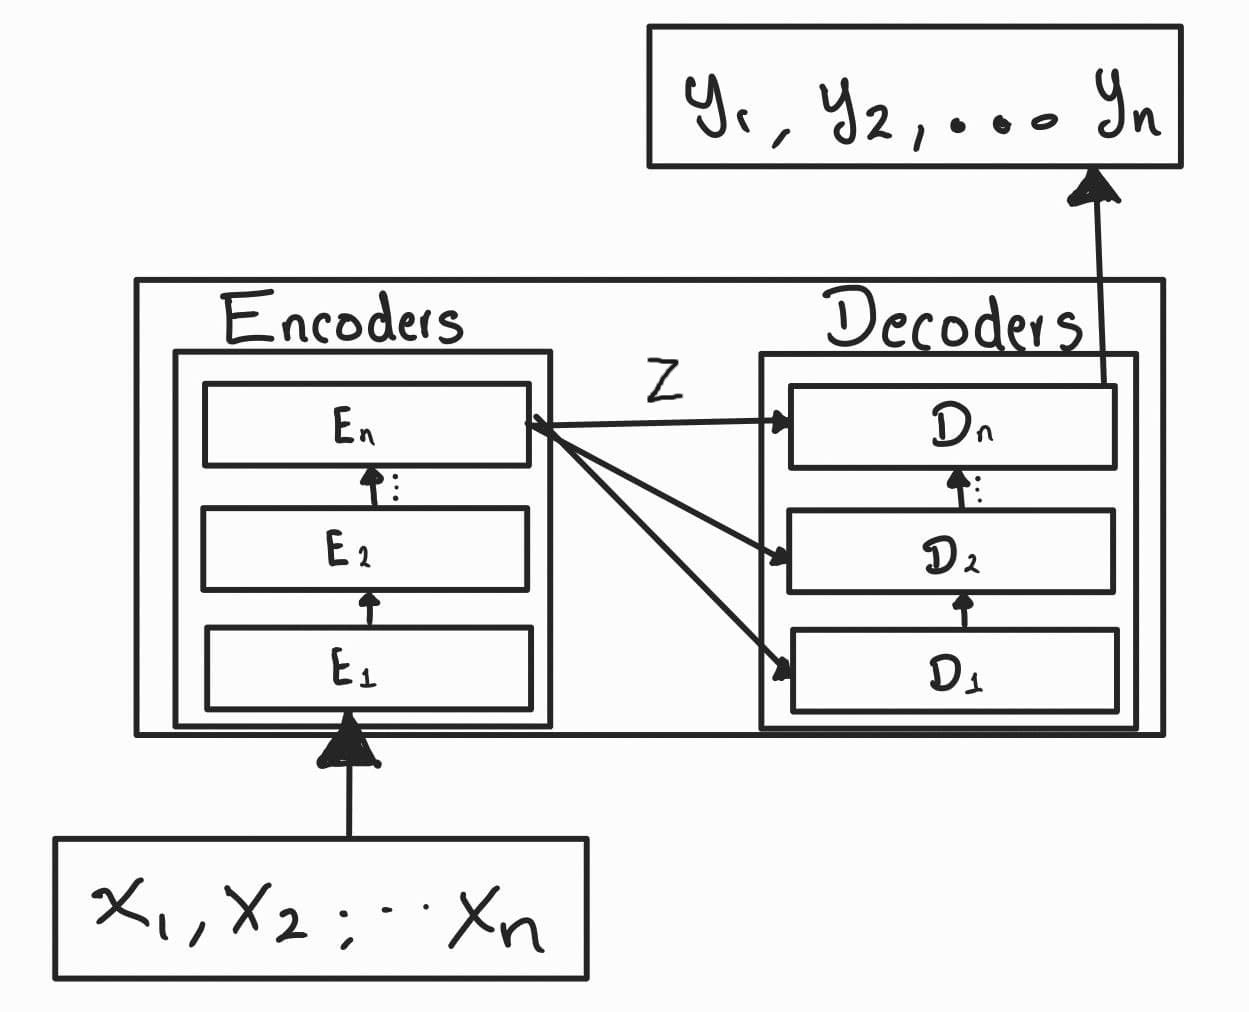
\includegraphics[width=0.4 \textwidth]{Chapters/2. Transformer/Figures/transformer/t_seq2seq.jpg}
    \caption{Modelo Transformer generalizado como modelo Secuencia a Secuencia}
    \label{fig:trans_seq2sqe}
\end{figure}


\subsection{El Codificador y Decodificador}

El \textit{Modelo Transformer} está formado por multiples codificadores  y decodificadores apilados e inter-conectados,
Como observamos en la figura \ref{fig:trans_seq2sqe}. El codificador consta de dos capas,
la primera de ellas aplica \textit{Self-Attention} múltiples veces sobre la misma entrada
(\textit{Multi-HeadSelf Attention}) y la segunda capa representada solo por una red
\textit{Feed-Forward} cuya entrada es la salida de la capa anterior.
Véase la figura \ref{fig:trans_encoder}.


\begin{figure}[ht!]
\centering
    \begin{minipage}{.4\textwidth}
        \centering
        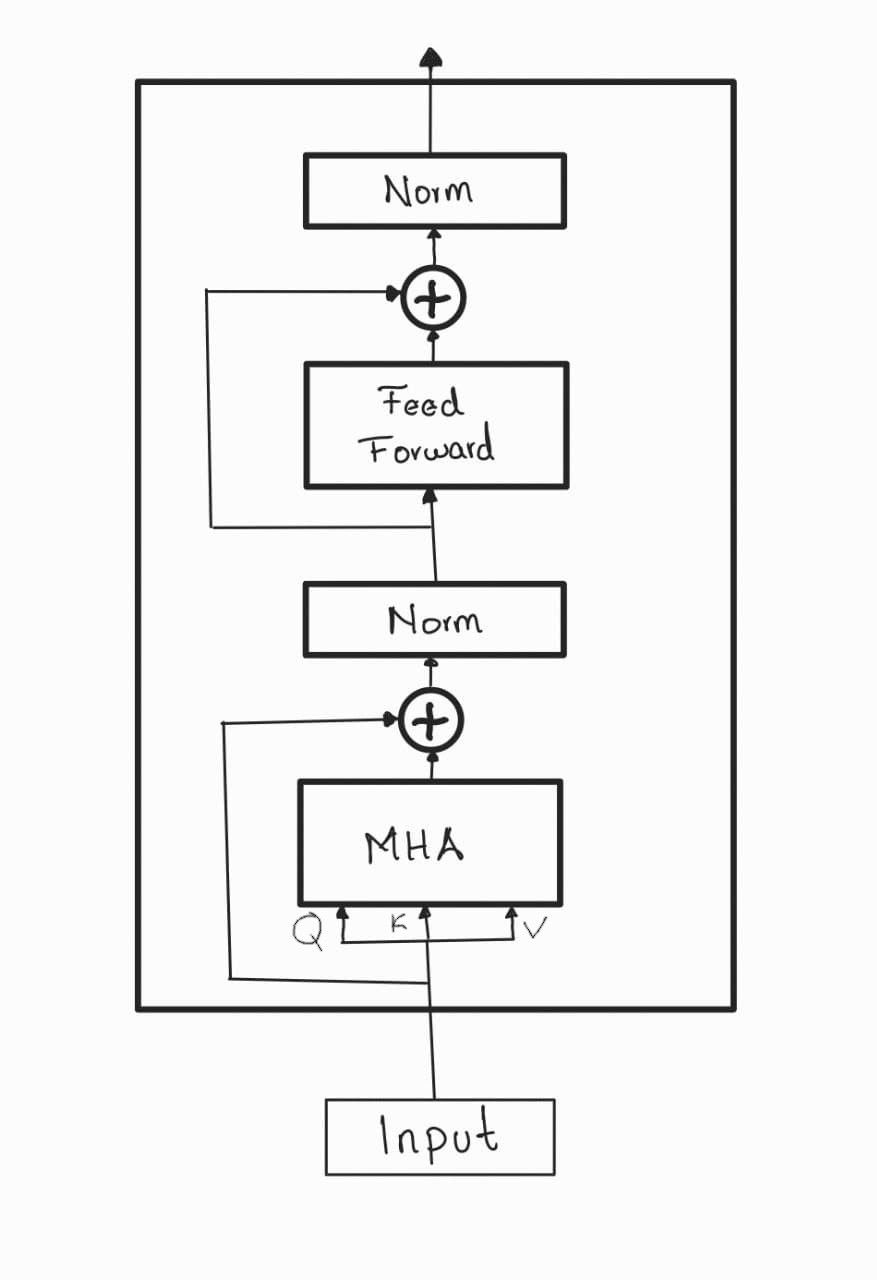
\includegraphics[width=0.7 \textwidth]{Chapters/2. Transformer/Figures/transformer/encoder.jpg}
    \end{minipage}
    \begin{minipage}{.5\textwidth}
        \begin{equation*}
            \begin{split}
                mha = MHA(X, X, X)\\
                norm = Norm( mha + X)\\
                f = FeedForward(norm)\\
                Encoder(X) = Norm(f + norm)
            \end{split}
            \label{eq:trans_enc}
        \end{equation*}
    \end{minipage}
    \caption{Etapa Codificadora del Modelo Transformer. Pseudocódigo}
    \label{fig:trans_encoder}
\end{figure}


El decodificador tiene una estructura similar al codificador con una etapa adicional intermedia
de \textit{Multi-Head Attention} aplicada sobre la salida de la pila de codificadores. También, la
primer capa de atención sufre un ligero cambio un su forma de operación, necesitando enmáscarar (al
momento en que se realiza el entrenamiento) la atención prestada del pasado al futuro. Esto es
debido a que el decodificador se encarga de generar una secuencia (en modo inferencia) uno a la vez
usando solamente la salida anterior y por tanto no tiene conocimiento de salidas futuras, observe
la figura \ref{fig:trans_te}.

\begin{figure}[ht!]
\centering
    \begin{minipage}{.4\textwidth}
        \centering
        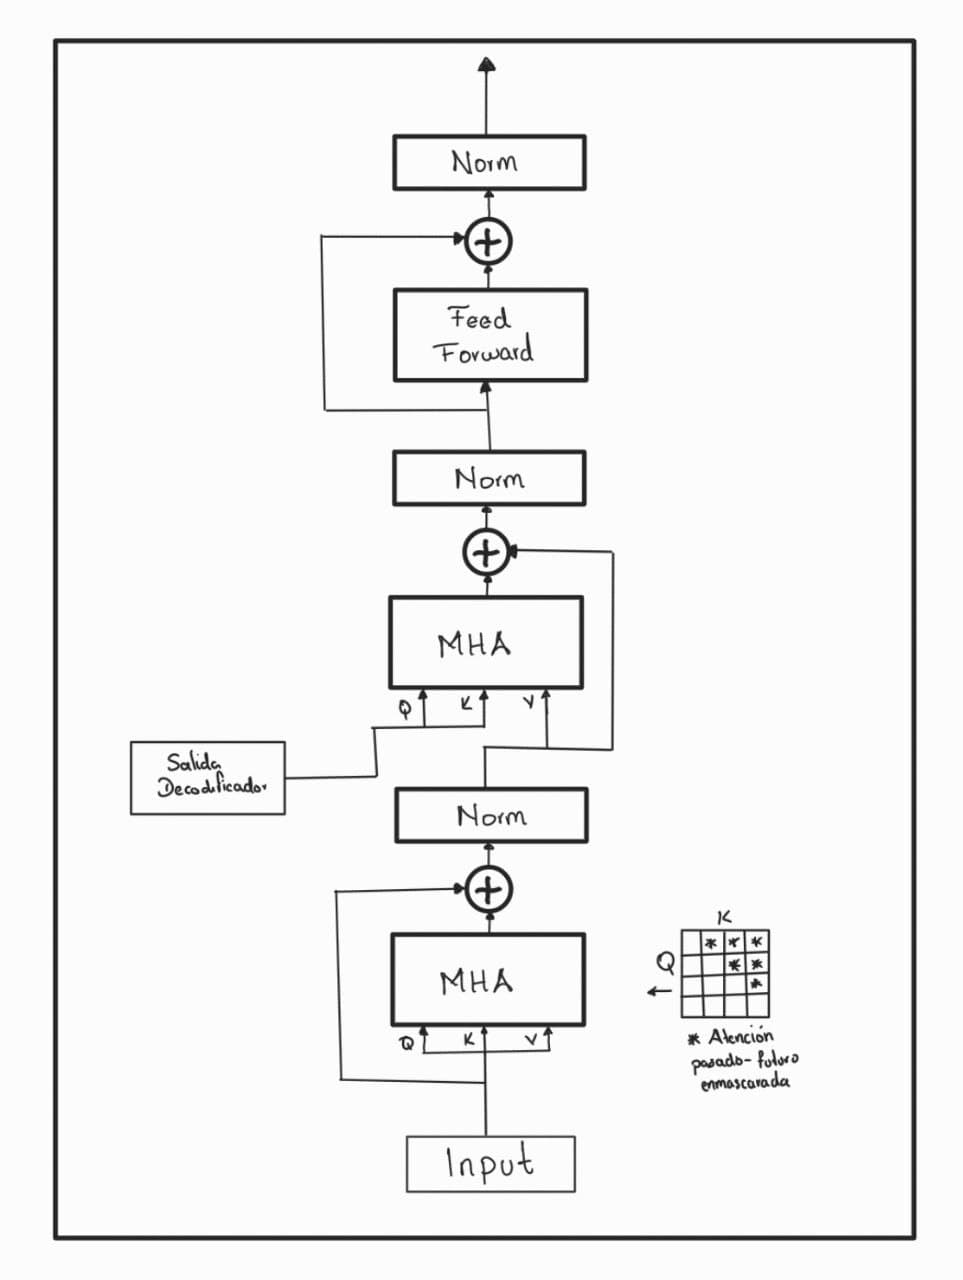
\includegraphics[width=1.0 \textwidth]{Chapters/2. Transformer/Figures/transformer/decoder.jpg}
    \end{minipage}
    \begin{minipage}{.5\textwidth}
        \begin{equation*}
            \begin{split}
                mha_1 = MHA(X, X, X)\\
                norm_1 = Norm( mha_1 + X)\\
                mha_2 = MHA(enc_{out}, enc_{out}, norm_1)\\
                norm_2 = Norm( mha_2 + X)\\
                f = FeedForward(norm_2)\\
                decoder(X) = Norm(f + norm_2)
            \end{split}
            \label{eq:trans_dec}
        \end{equation*}
    \end{minipage}
    \caption{Etapa Decodificadora del Modelo Transformer. Pseudocódigo}
    \label{fig:trans_decoder}
\end{figure}


\begin{figure}[ht!]
    \centering
    \begin{subfigure}[b]{0.49\textwidth}
        \centering
        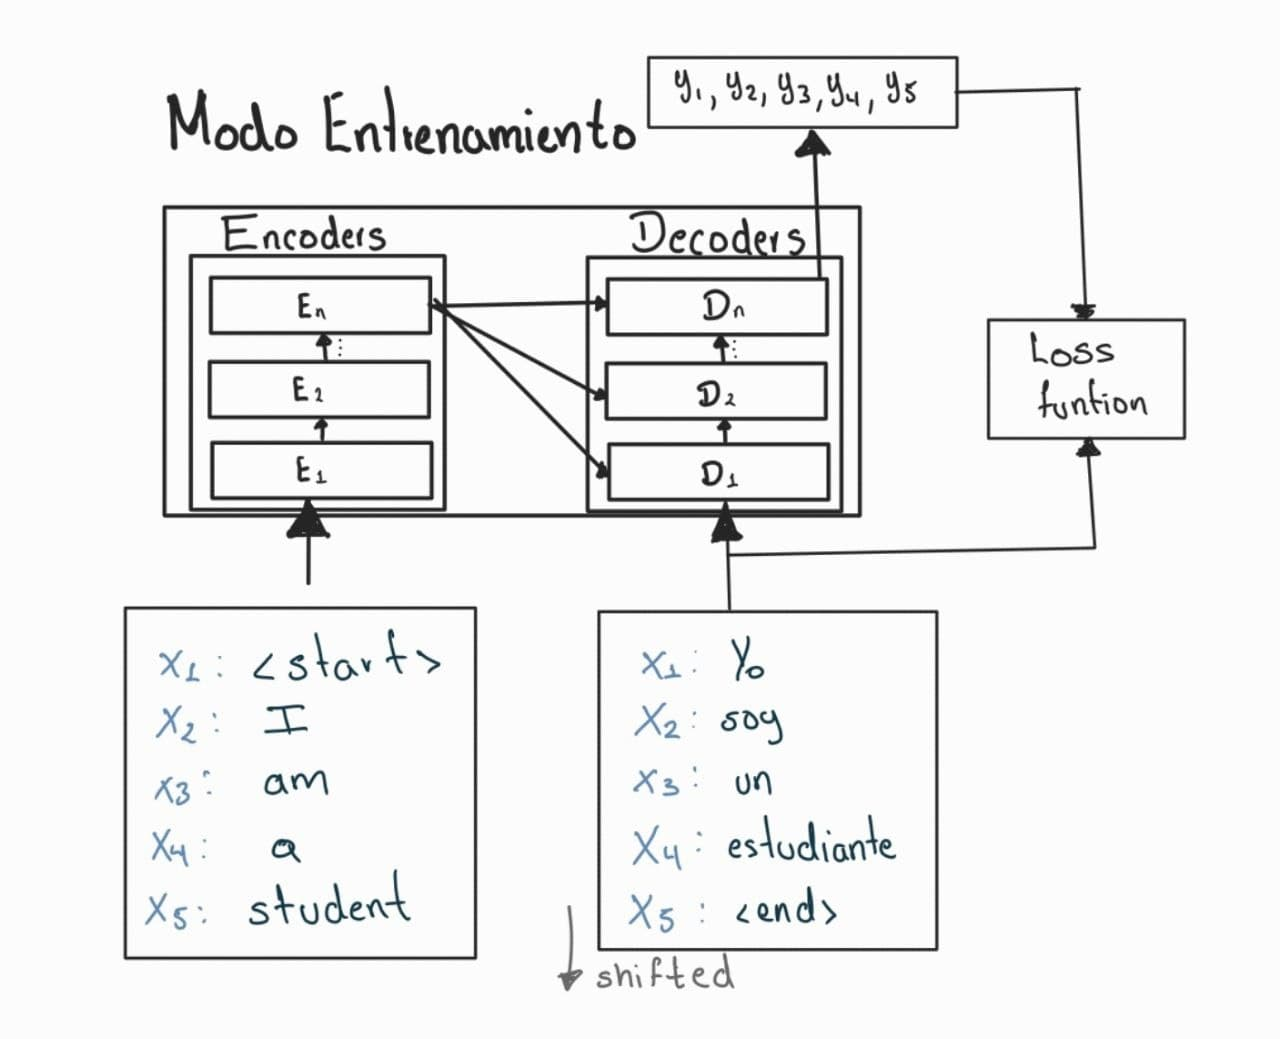
\includegraphics[width=1.0 \textwidth]{Chapters/2. Transformer/Figures/transformer/train.jpeg}
        \caption{Transformer modo entrenamiento. Las entradas en el decodificador son recorridas un
                 elemento en el futuro, con el fin de que aprende a predecir la siguiente palabra
                 dado un contexto previo y las salidas actuales en el momento de la evaluación.}
        \label{fig:trans_train}
    \end{subfigure}
    \begin{subfigure}[b]{0.49\textwidth}
        \centering
        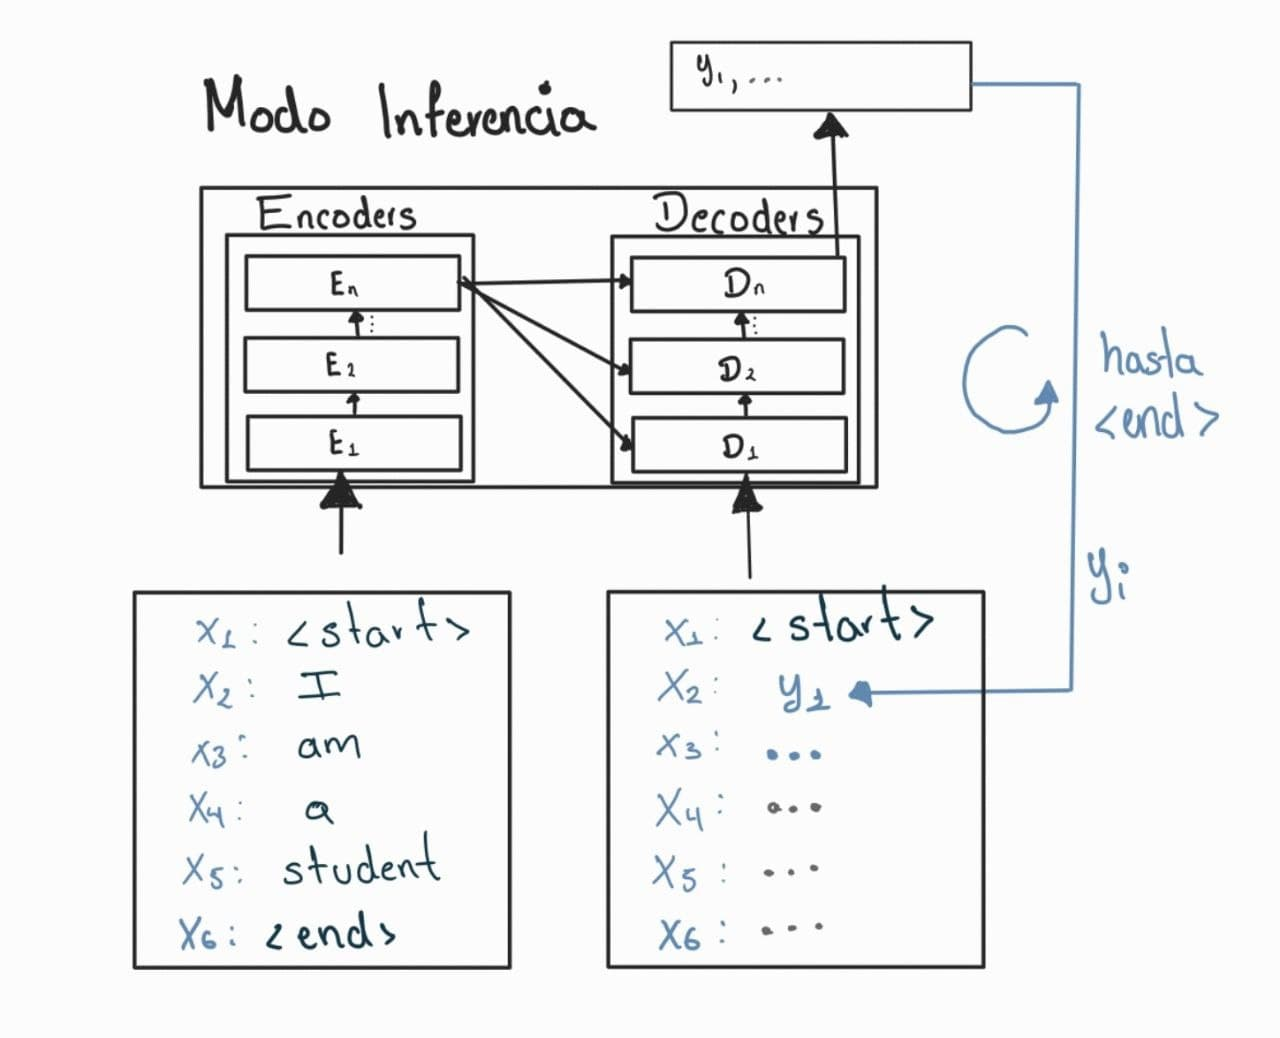
\includegraphics[width=1.0 \textwidth]{Chapters/2. Transformer/Figures/transformer/inference.jpg}
        \caption{Transformer modo inferencia. El decodificador funciona como un modelo auto-regresivo,
        usa sus predicciones hasta el tiempo $t$ para obtener el siguiente valor. En la primer iteración
        el decoder solo recibe el token de inicio de oración $<start>$ por lo que podrá predecir la primer
        palabra de la oración gracias a que fue entrenado con un desplazamiento hacia el futuro. En la siguiente
        iteración el nuevo token predicho es agregado como entrada al decodificador. El decodificador
        termina su predicción en el momento que el token $<end>$ es obtenido.}
        \label{fig:trans_eval}
    \end{subfigure}
    \caption{Esquema de entrenamiento e inferencia del modelo Transformer en un problema de
             Machine Translation.}
        \label{fig:trans_te}
\end{figure}


\subsection{Multi-Head Self-Attention} \label{section-mha}

En la sección \ref{section:att} se detalla una generalización de la atención y diversas variantes usadas
a lo largo de la literatura. El modelo original que introdujo a los Transformers usa en especial la variante
\textit{Scaled Dot-Product Attention}\cite{Vaswani}:

\begin{equation}
    Attention(q, k, v) = softmax(\frac{q k^\top}{\sqrt{d_k}}) v
    \label{eq:trans_att_gen}
\end{equation}

El Transformer está basado en la idea de de aplicar atención multiples veces, al usar varias cabezas
de atención, Multihead-Self-Attention (MHA), permite  al modelo conjuntamente atender a información
en distintas posiciones desde $h$ diferentes subespacios de representación. \ref{eq:mha}

\begin{equation}
    mha(Q, K, V) = Concat(head_1,head_2,head_3,..., head_h)W^O
    \label{eq:mha}
\end{equation}

Todas las cabezas de atención son concatenadas y resumidas para ser devueltas a las dimensiones del
espacio de entrada original, principalmente para mantener consistencia en las dimensiones de usadas
en cada etapa de codificación y decodificación del modelo a través de $W^O \in \mathbb{R}^{hd_v \times d_m}$.
$W^O$ es entrenado conjuntamente para aprender a resumir la información capturada por cada cabeza de
atención. $Q, K \in \mathbb{R}^{n \times d_{m}}$ y $V \in \mathbb{R}^{n \times d_{v}}$ es la representación
consulta, clave y valor de los embeddings de entrada de cada capa de atención del codificador y
decodificador como se observa en las figuras \ref{fig:trans_encoder} \ref{fig:trans_decoder}.
$n$ es el tamaño de la secuencia, $d_m$ y $d_v$ son los tamaño del embedding y $h$ el número de
cabezas de atención.

En el caso del modelo transformer tenemos un conjunto embeddings sobre las cuales se aplica atención,
si bien, no representan necesariamente las consultas, llaves, y valores utilizados para la atención
generalizada, podemos obtener estas representaciones transportándolos a sus espacios respectivos a través de alguna
transformación aprendida conjuntamente con el entrenamiento del modelo.

Por tanto, para el conjunto de Embeddings  $E_Q \in \mathbb{R}^{n \times d_m}$,
$E_K \in \mathbb{R}^{n \times d_m}$ y $E_V \in \mathbb{R}^{n \times d_v}$ donde $n$ es el número
embeddings, $d_m$ y $d_v$ son las dimensiones de cada uno, la atención en cada cabeza $i$ se calcula
como:

\begin{equation}
    \begin{split}
        Q_i = E_Q W_i^Q\\
        K_i = E_K W_i^K\\
        V_i = E_V W_i^V\\
    \end{split}
\end{equation}

\begin{equation}
\begin{split}
    head_i = Attention(Q_i, K_i, V_i) = softmax\Big(\frac{Q_i K_i^T}{\sqrt{d_k}}\Big) V_i
    \label{eq:trans_att}
\end{split}
\end{equation}

donde $W_i^Q$, $W_i^K$ $\in \mathbb{R}^{d_m \times d_k}$, $W_i^V$ $\in \mathbb{R}^{d_m \times d_v}$
y $d_k=d_v=d_m/h$.

el término de escalamiento $\sqrt{d_k}$ ayuda a evitar que la magnitud de los productos puntos calculados
entre cada consulta y llave crezcan demasiado, y que la función $softmax$ pueda ser más estable al evitar
regiones donde los gradientes son muy pequeños\cite{Vaswani}.


\subsection{Información Posicional}

En los modelos basados en \textit{Redes Recurrentes} la información se procesan uno a uno en cada paso de
tiempo. Los modelos basados en \textit{Transformers} procesan la información en conjunto, perdiendo
la noción de la temporalidad de los datos. Una solución es agregar dicha información perdida a través
de vectores que codifiquen el tiempo/posición de los datos sumándolos con los vectores de embeddings.
Estos vectores llamados \textit{Positional Encodings} \cite{DBLP:journals/corr/GehringAGYD17} siguen
un patrón en específico
que el modelo aprende a identificar y lo ayuda a determinar la posición de cada elemento de la secuencia
y por tanto calcular a qué distancia se encuentra cada uno de los demás.

Por lo regular se usa una onda senoidal y cosenoidal para lugares pares e impares, formando una progresión
geométrica desde $2\pi$ hasta $10000 \cdot 2\pi$ \ref{eq:trans_pos_enc}:

\begin{equation}
    \begin{split}
        PE(pos, 2i) = \sin(pos/10000^{2i/d_m})\\
        PE(pos, 2i+1) = \cos(pos/10000^{2i/d_m})
    \end{split}
    \label{eq:trans_pos_enc}
\end{equation}


\begin{figure}[ht!]
    \centering
    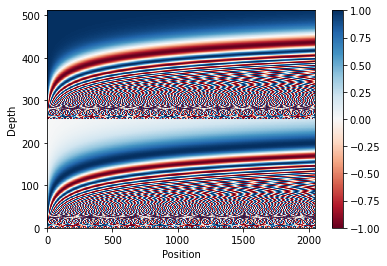
\includegraphics[width=0.5 \textwidth]{Chapters/2. Transformer/Figures/transformer/pos_enc.png}
    \caption{2000 Vectores de Positional Encoding con dimensiones de embedding=500.}
    \label{fig:trans_pos_enc}
\end{figure}

Poner una figura completa de todo el esquema del Transformer

\subsection{Problemas típicos en el entrenamiento de Transformers}

\subsubsection{Learning Rate WarmUp y Layer Normalization}

A pesar de que la arquitectura del modelo Transformer no es tan compleja, puesto que tanto el
codificador como el decodificador están formados por pilas de capas de atención y MLP, el
entrenamiento de este tipo de modelos muchas veces no resulta tan trivial. Regularmente requiere de
una combinación de técnicas para lograr su convergencia a valores aceptables y en conjunto con una
gran cantidad de datos, tamaños de lotes de procesamiento grandes y una gran cantidad de tiempo
de procesamiento en gpu \cite{DBLP:journals/corr/abs-1804-00247}.

\textit{Learning Rate WarmUp} es una de las primeras técnicas usadas y descritas en el proceso de
entrenamiento por \citeauthor{Vaswani}. Usando el algoritmo Adam como optimizador se varía el factor
de aprendizaje de acuerdo a la fórmula:

\begin{equation}
    lrate = d_{m}^{-0.5} \vdot \min\big(step\_num^{-0.5}, step\_num \vdot warmup\_steps^{-0.5} \big)
\end{equation}

En el esquema anterior, más conocido como \textit{Noam-Warmup}, el modelo original es entrenado
incrementando linealmente el factor de aprendizaje en los primeros $warmup\_steps=4000$ pasos.
Posteriormente, decrementa propocionalmente al inverso del la raíz cuadrada del paso $step\_num$
actual, véase la figura \ref{fig:noam}.

\begin{figure}[ht!]
    \centering
    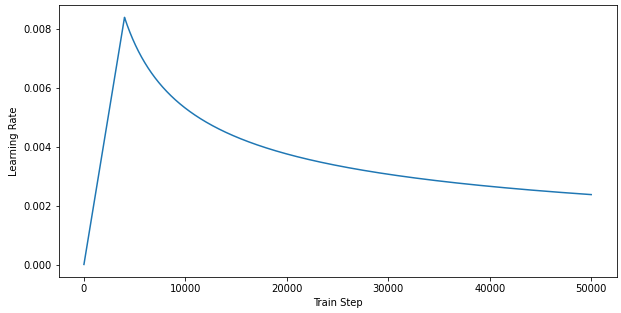
\includegraphics[width=0.5 \textwidth]{Chapters/2. Transformer/Figures/transformer/noam.png}
    \caption{Noam-Warmup con $warmup\_steps=4000$ y $d_{m} = 512$}
    \label{fig:noam}
\end{figure}

Si bien, la razón por la que funciona este tipo de técnica no está del todo claro, se presume que usar
\textit{Learning Rate WarmUp} ayuda a reducir la varianza del factor de aprendizaje adaptativo durante
las primeras etapas del entrenamiento del modelo. \citeauthor{DBLP:journals/corr/abs-1908-03265}
demostraron que el segundo momento del algoritmo
de Adam durante etapas tempranas de optimización es proporcional a una integral divergente, lo que
provoca las actualizaciones inestables, llevando al
modelo fuera de las regiones donde un mejor mínimo existe. Con esto en mente
\citeauthor{DBLP:journals/corr/abs-1908-03265} proponen el algoritmo de optimización
\textit{RAdam} (Rectified Adam) como una alternativa a usar \textit{Learning Rate WarmUp} y mitigar
este efecto durante la fase inicial del entrenamiento de los modelos.

El \textit{Learning Rate WarmUp}
comúnmente es usado en conjunto con algoritmos de optimización estocásticos como \textit{RMSprop} o
\textit{Adam}. En vez configurar el \textit{factor de aprendizaje} $\alpha$ con un decremento
constante, la estrategia de \textit{Learning Rate WarmUp} configura este factor con valores muy
pequeños en los primeros pasos de entrenamiento. Durante las primeras etapas del entrenamiento
el factor de aprendizaje es incrementado hasta un límite que es ligeramente superior o inferior al valor
inicial de $\alpha$ del optimizador usado y posteriormente es  decrementado
progresivamente hasta la convergencia del modelo.

Así, en cada paso del algoritmo de optimización el cuál está parametrizado por el factor de aprendizaje
$\alpha$, puede ser aplicado un factor de \textit{warmup} $\omega \in [0,1]$ que sirve para reducir
$\alpha$ y a la vez el paso de optimización en cada tiempo, replazando $\alpha_t = \alpha \omega_t$.
La forma mas sencilla es usar un factor \textbf{linear warmup} parametrizado por un periodo de
\quotes{calentamiento} $\tau$.

\begin{equation}
    \omega_t^{linear, \tau} = \min\big(1, \frac{t}{\tau} \big)
    \label{eq:warn_linear}
\end{equation}

\citeauthor{DBLP:journals/corr/abs-1910-04209} proponen 3 formas de aplicar la técnica de \textit{warmup}:

\textbf{Exponential warmup} aplica un decaimiento exponencial

\begin{equation}
    \omega_t^{expo, \tau} = 1 - \exp(- \frac{1}{\tau} t)
    \label{eq:warn_expo}
\end{equation}

recomienda elegir $\tau = (1 - \beta_2)^{-1}$ tal que no se tan diferente del segundo momento de
corrección de bias del algoritmo de \textit{Adam} $\beta_2$.

\begin{equation}
    \omega_t^{expo, untuned} = 1 - \exp(- (1 - \beta_2) t)
    \label{eq:warn_expo_untened}
\end{equation}

Similar al decaimiento exponencial proponen usar \textit{linear warmup} sobre
$\tau = 2 (1 - \beta_2)^{-1}$ iteraciones para preservar un efecto similar de des-aceleración
con el paso del tiempo.

\begin{equation}
    \omega_t^{linear, untuned} = \min\big(1, \frac{1 - \beta_2}{2} t \big)
    \label{eq:warn_linear_untuned}
\end{equation}

\begin{figure}[ht!]
    \centering
    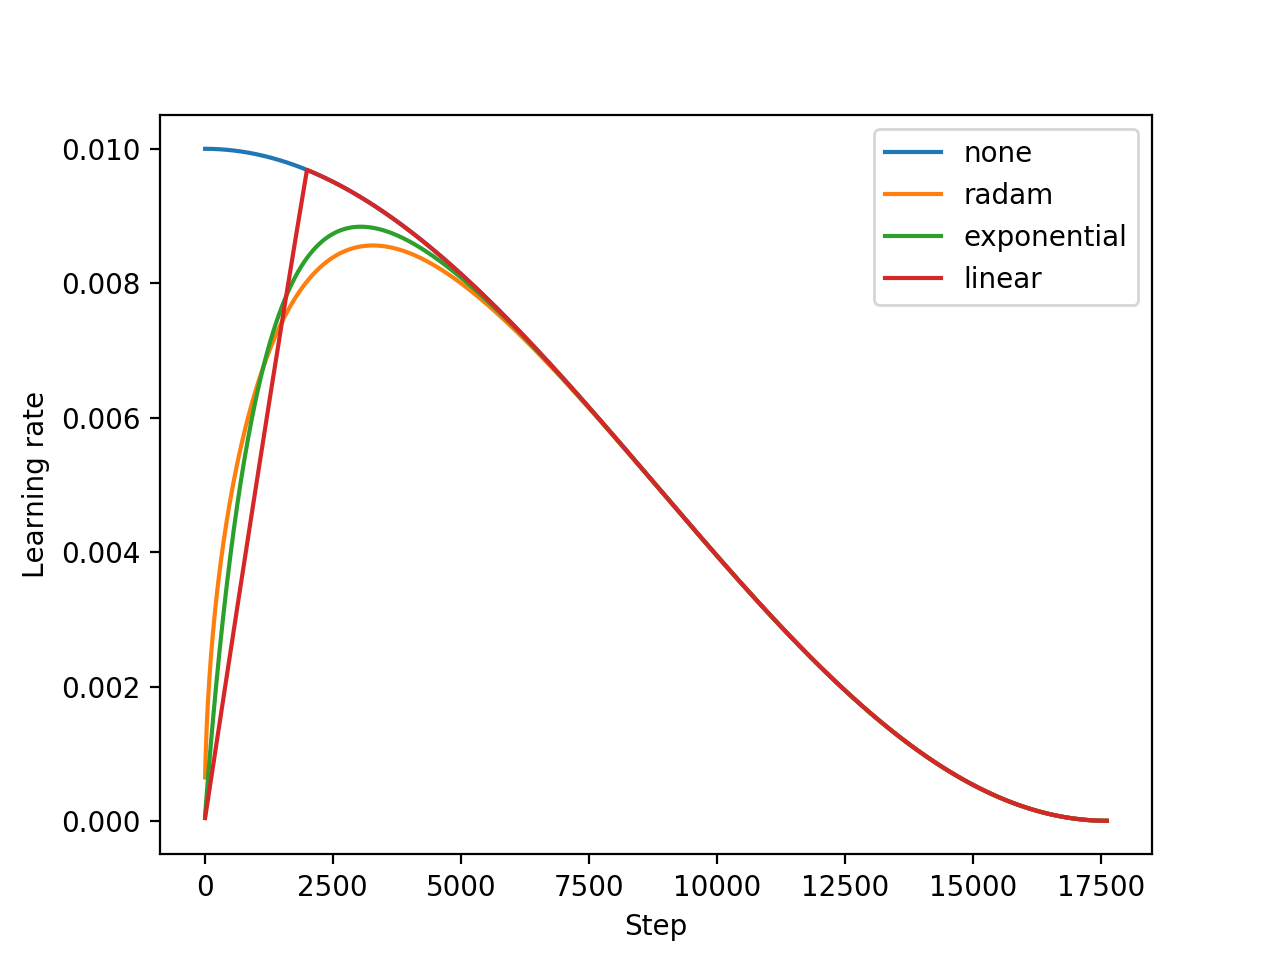
\includegraphics[width=0.5 \textwidth]{Chapters/2. Transformer/Figures/transformer/warmups.png}
    \caption{Learning rate sobre X 18000 iteraciones usando RAdam y lineal, exponencial warmup con Adam}
    \label{fig:warmup}
\end{figure}


Por otro lado, \citeauthor{pmlr-v119-huang20f} mencionan que usar la técnica de \textit{Learning Rate WarmUp}
para mitigar la varianza del optimizador Adam no es del todo la solución y que el problema radica
precisamente en la arquitectura del modelo Transformer, principalmente en las capas de normalización
\cite{DBLP:journals/corr/abs-1804-09849} \cite{DBLP:journals/corr/abs-2002-04745}. En particular
\citeauthor{DBLP:journals/corr/abs-2002-04745} encuentran que para un modelo Transformer de cualquier
tamaño con capas de normalización entre bloques residuales (\textit{Post-LN Transformer}), la escala
de la norma del gradiente que incide en la última capa de normalización permanecen igual al no depender
de la cantidad de bloques del transformer. Por el contrario, si la capa de normalización es colocada
justo antes de la conexión residual (\textit{Pre-LN Transformer}) la magnitud de la norma del
gradiente decrece conforme el tamaño del modelo incrementa, guiando así, al problema de desvanecimiento de
gradiente. \citeauthor{pmlr-v119-huang20f} proponen eliminar las capas de normalización del modelo
Transformer que en conjunto con la inestabilidad del algoritmo de optimización de Adam provocan la
dificultad de entrenamiento durante desde las primeras etapas. Para ello, estandarizan la siguiente
inicialización (\textit{T-Fixup}) de pesos del modelo, permitiendo evitar la etapa de \textit{WarmUp}
y las capas de normalización en el Transformer. La figura \ref{fig:t-fixup} muestra una comparativa
de los histogramas usando la inicialización \textit{T-Fixup} e usar el algoritmo de Adam con y sin
etapa de \textit{Warmup}:

\begin{itemize}
    \item Aplicar initialization tipo \textit{Xavier} para todos los pesos del modelo.
          Excepto el proceso de generación de embedding adecuados al tamaño del modelo $d_m$.
    \item Usar una inicialización tipo \textit{Gaussiana} con $\mathbb{N}(0, d_m^\frac{1}{2})$ para
          los pesos de generación de embeddings.
    \item Escalar las matrices $W_i^V$ y $W^O$ en cada bloque de atención en el decodificador, los
          pesos en de cada capa MLP del decodificador y los pesos de generación de embeddings tanto
          del codificador como decodificador por $9N^{-\frac{1}{4}}$ donde $N$ es el número de bloques
          del Transformer.
    \item Escalar las matrices $W_i^V$ y $W^O$ de cada bloque de atención del codificador y los pesos
          de cada capa de MLP del codificador por $0.67N^{-\frac{1}{4}}$
\end{itemize}

\begin{figure}[ht!]
    \centering
    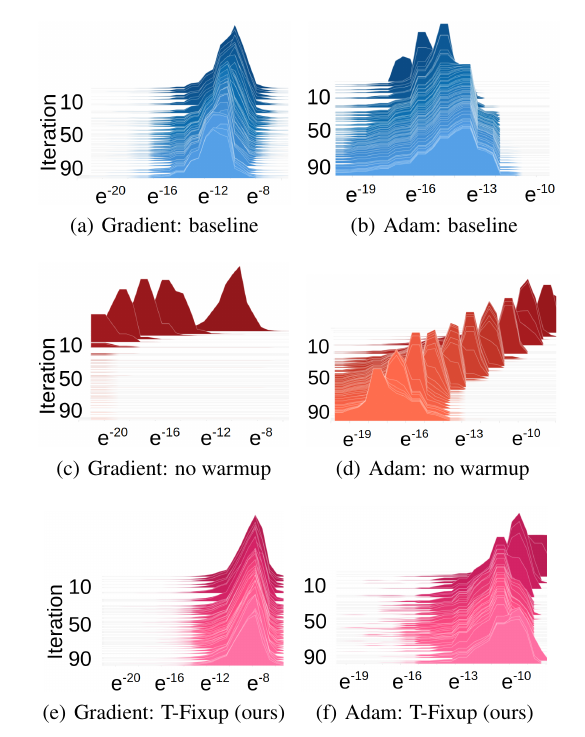
\includegraphics[width=0.5 \textwidth]{Chapters/2. Transformer/Figures/transformer/tfixup.png}
    \caption{Histograma de gradientes del Algoritmo Adam con y sin etapa de \textit{WarmUp} y
    usando inicialización \textit{T-Fixup}. Imagen original de \citeauthor{pmlr-v119-huang20f}}
    \label{fig:t-fixup}
\end{figure}

\subsubsection{Cálculo de la Atención}

Además de lo específico y delicado del entrenamiento del Modelo Transformer su costo en tiempo
computacional y de memoria también representa un serio problema a la hora de optimizar e inferir.
Debido principalmente a que en el proceso de atención debe focalizar cada token con respecto a todos
los demás, lo que lleva a que su complejidad crezca cuadráticamente con respecto a el tamaño de la
secuencia.

Varías técnicas han sido propuestas para reducir este problema, muchas de ellas involucran en reducir
la atención a vecindades de representaciones, aproximar la matriz de atención con otras matrices de
transformaciones a través de kernels o sustituir completamente la operación \textit{softmax}
por otra función.

\textbf{Atención de vecindades}:

\citeauthor{DBLP:journals/corr/abs-1802-05751} particionan la información de las representaciones de
las consultas asignándolos a diferentes bloques de memoria, restringiéndose a vecindarios locales
alrededor de cada consulta. Principalmente basados en cómo las redes convolucionales trabajar. Sin
embargo esta solucion es parcial y solo aplicable a secuencias de datos con relaciones cortas, cómo
imágenes.

\citeauthor{DBLP:journals/corr/abs-1904-10509} factorizan la matriz de atención para reducir su complejidad
de $O(n^2)$ a $O(n\sqrt(n))$ por medio de matrices ralas, separando la atención a través de diferentes
pasos al parametrizar la atención por una conectividad de distintos patrones elegidos previamente bajo el supuesto
de que las matrices de atención son ralas, puesto que no contienen dependencias de relevancia
sobre representaciones distantes como se observa en la imagen \ref{fig:att-spar}.

\begin{figure}[ht!]
    \centering
    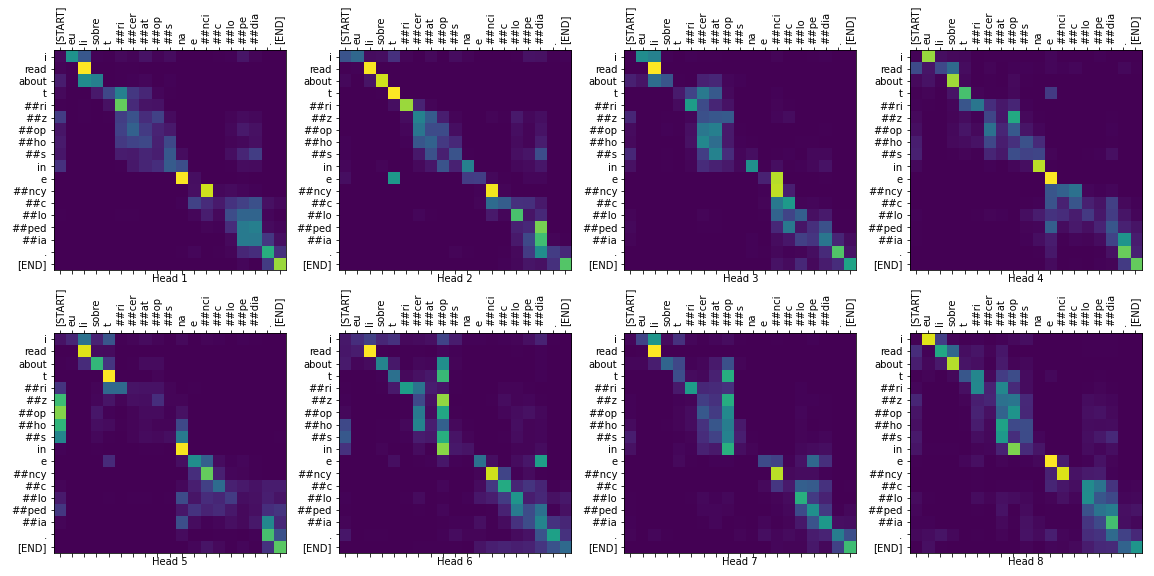
\includegraphics[width=0.7 \textwidth]{Chapters/2. Transformer/Figures/transformer/head_sparsity.png}
    \caption{Visualización de 8 cabezas de atención sobre una tarea de Machine-Translation. Las
    matrices de atención tienden a ser ralas al tener carencia de relaciones relevantes entre diversas
    representaciones a distancias lejanas.}
    \label{fig:att-spar}
\end{figure}

\citeauthor{DBLP:journals/corr/abs-1905-07799} proponen reducir el ancho de la atención basándose en
que cada representación no necesita prestar atención sobre todas las demás sino que debería ser
adaptativo. Así, para cada cabeza de atención se agrega una función de enmascaramiento que controla
la flexibilidad del ancho una ventana. La ventana formada cambia dinámicamente de tamaño
dependiendo de la representación en cuestión.
\citeauthor{DBLP:journals/corr/abs-2004-05150} siguen un estrategia similar, implementado
atención local con ventanas dilatadas distintas para cada cabeza, permitiendo atender contextos menos
locales en cada ocasión y atención global sobre preseleccionados localizaciones. Dada la dificultad de
su implementación sin usar ciclos para iterar sobre los elementos seleccionados a atender, implementan
su propio kernel en \textit{CUDA} con las operaciones optimizadas para realizar esta tarea.

\citeauthor{DBLP:journals/corr/abs-1901-02860} mencionan que si el problema es el procesamiento de
grandes secuencias por qué no dividirlas en secuencias más pequeñas y procesarlas individualmente
y así evitar usar grandes cantidades de memoria en su procesamiento. El principal problema de este
enfoque es que cada secuencia es procesada individualmente y la información de previas secuencias es
ignorada evitando que esta fluya a través de las próximas secuencias. Para solucionar este
inconveniente introducen un mecanismo de recurrencia en la arquitectura del transformer. Durante el
entrenamiento (véase la figura \ref{fig:trans-xl}) un estado oculto es calculado de las secuencias previas y guardado
en memoria para extender el contexto al momento de procesar la siguiente secuencia. Durante el
proceso de evaluación, el resultado de las operaciones del transformer pueden ser reusado y no
calculado nuevamente desde cero, permitiendo reducir considerablemente el tiempo de evaluación.

\begin{figure}[ht!]
    \centering
    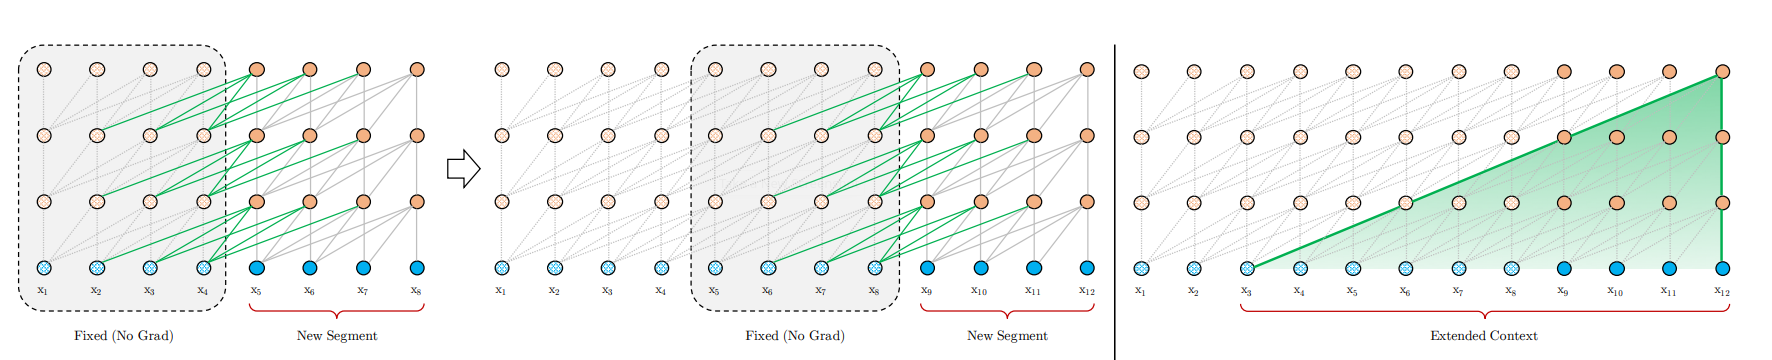
\includegraphics[width=0.8 \textwidth]{Chapters/2. Transformer/Figures/transformer/trans-XL.png}
    \caption{Transformer-XL. Para tratar con secuencias largas divide el proceso en secuencias más
             cortas creando estados ocultos intermedios y usandolos en el cálculo de las próximas
             secuencias. Figura obtenida de \cite{DBLP:journals/corr/abs-1901-02860}.}
    \label{fig:trans-xl}
\end{figure}

\citeauthor{DBLP:journals/corr/abs-2001-04451} reducen el problema de realizar la operación de softmax
sobre toda la matriz $Q_i K_i^\top$ a calcularlo individualmente por cada consulta $q_j$, guardando
solo una vez en memoria este valor en cada iteración y recalculándolo cuando se necesite de nuevo
al utilizar \textit{Back-Propagation} usando de capas reversibles. Si bien, computacionalmente es
más costoso permite usar mucho
menos memoria que la solución original. Por otro lado, dado que el resultado de la función softmax
depende en mucho mayor medida en los elementos dominantes de la matriz, solo es necesario fijarse en
las llaves más cercanas a la consulta en cuestión. \textit{LSH} (\textit{Local Sensitive Hashing})
resuelve este problema permitiendo encontrar rápidamente los vecinos más cercanos en espacios de altas
dimensiones, con la  restricción de que $W_i^Q = W_i^K$ dado que se necesita conservar la
similaridad entre consultas y llaves, algo que sería más dificil si sus matrices de proyección
$W_i^Q$ y $W_i^K$ fuesen muy distintas.

\textbf{Aproximaciones a la Atención original}:

También \citeauthor{DBLP:journals/corr/abs-1906-11024} proponen un modelo para compartir pesos de capas
adyacentes (Shared Attention Network - SAN).
Cada $\pi$ capas continuas en el codificador comparten la misma matriz de atención y en el
decodificador se comparte la proyección de los pesos de atención sobre la representación de los
valores $V_i$, en otras palabras se comparte directamente la cabeza de atención $head_i$. Dado que no
es tan fácil conocer que capas deben compartir pesos, establecen un proceso iterativo
de entrenamiento basados en calcular que tan diferentes son las capas del transformer usando
la \textit{Divergencia de Jensen-Shannon}. Si la similaridad entre dos capas es mayor a cierto umbral
se indica que dichas capas deben compartir pesos. Se repite un nuevo entrenamiento y se calcula
nuevamente la similaridad entre capas, y así sucesivamente hasta convergencia. Podemos notar que este
proceso de entrenamiento y ajuste de pesos es muy costoso, un nuevo entrenamiento es requerido por
cada ajuste de compartición de pesos, pero el modelo resultante
es menos complejo y el tiempo en modo de evaluación o inferencia se ve reducido considerablemente.

\citeauthor{DBLP:journals/corr/abs-2006-04768} bajo la hipótesis de que la matriz de atención tienen
rango mucho menor que $n$ proponen obtener los valores de cada cabeza haciendo una aproximación a ella.
Para ello, se hace uso de dos matrices entrenables conjuntamente con el modelo, $E$ y $F$
$\in \mathbb{R}^{n \times k}$ con $k \ll n$, tal que,
$head_i = softmax(\frac{Q_i (E_i K_i)}{\sqrt{d_m}}) F_iV_i$. Con ello la dimensión correspondiente al
tamaño de las secuencias se ve reducido bajo el supuesto que podemos representar la información
secuencial en un espacio más pequeño sin gran pérdida de información.

\citeauthor{DBLP:journals/corr/abs-2009-14794} por el contrario descomponen la operación de atención
sobre los valores $head = softmax(\frac{QK^\top}{\sqrt{d_k} V})$ en una multiplicación matricial más simple
$head = Q'k'^\top V$ con $Q'$ y $k'^\top \in \mathbb{R}^{n \times r}$ y $r<=n$.
Para ello construyen $Q'$ y $k'$ como dos matrices usando kernels tal que su producto forma una
aproximación a la función softmax aplicada al producto de $Q$ y $K$. Notemos que con ello podemos
reducir el costo computacional y en
memoria simplemente reduciendo el producto $Q'(k'^\top V)$ de derecha a izquierda.

Finalmente autores como \citeauthor{DBLP:journals/corr/abs-2105-03824} remplazan completamente
el bloque de \textit{Multihead Attention} con bloques que aplican operaciones de Transformada de
Fourier o lo largo de la dimensión de los  embeddings y de las secuencias. Probando que el usar
\textit{FFT} (Fast Fourier Transform) es suficiente para abstraer y modelar las relaciones. Y como
\citeauthor{DBLP:journals/corr/abs-2108-09084} que cambian la atención entre todas las consultas
y llaves por una sola con todas las llaves. Para esto, a través de atención sumarizan todos las
consultas en una consulta global. Este proceso es repetido con las llaves y valores como se observa
en la figura \ref{fig:fast-former}

\begin{figure}[ht!]
    \centering
    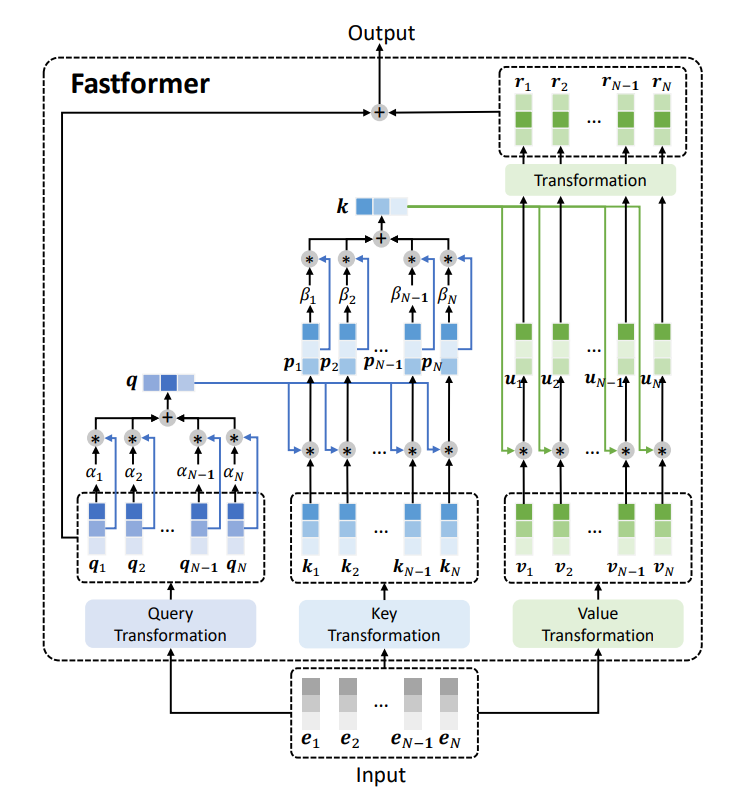
\includegraphics[width=0.6 \textwidth]{Chapters/2. Transformer/Figures/transformer/fastformer.png}
    \caption{Fast-Former. Remplaza la atención tradicional del  transformer por una iterativa. En
             cada paso crea una consulta y clave global usando atención sobre estos mismos.
             Figura obtenida de \cite{DBLP:journals/corr/abs-2108-09084}}
    \label{fig:fast-former}
\end{figure}
